\documentclass[crop,tikz]{standalone}
\usetikzlibrary{%
    arrows,
    arrows.meta,
    automata,
    backgrounds,
    calc,
    decorations.pathreplacing,
    fit,
    matrix,
    positioning,
    scopes,
    shadows
}
\usepackage[linguistics]{forest}
\usepackage[charter]{mathdesign}
\tikzset{headarrow/.style = {-{Latex[length=.5em]}}}

\begin{document}
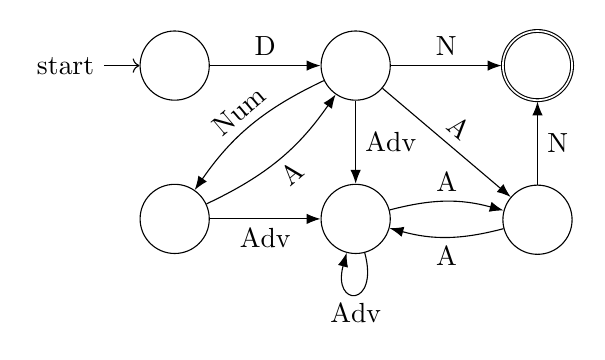
\begin{tikzpicture}
    \node[state,initial] (n-0-0) at (0,0) {};
    \node[state] (n-0-1) [right=4em of n-0-0] {};
    \node[state,accepting] (n-0-2) [right=4em of n-0-1] {};
    \foreach \x/\newx in {0/3, 1/4, 2/5}
        \node[state] (n-0-\newx) [below=3em of n-0-\x] {};

    \draw[headarrow] (n-0-0) to node [above] {D} (n-0-1);
    \draw[headarrow] (n-0-1) to node [above] {N} (n-0-2);
    \draw[headarrow] (n-0-1) to [bend right=15] node [above,sloped] {Num} (n-0-3);
    \draw[headarrow] (n-0-1) to node [right] {Adv} (n-0-4);
    \draw[headarrow] (n-0-1) to node [above,sloped] {A} (n-0-5);
    \draw[headarrow] (n-0-3) to [bend right=15] node [below,sloped] {A} (n-0-1);
    \draw[headarrow] (n-0-3) to node [below] {Adv} (n-0-4);
    \draw[headarrow] (n-0-4) [loop below] to node [below] {Adv} (n-0-4);
    \draw[headarrow] (n-0-4) to [bend left=15] node [above] {A} (n-0-5);
    \draw[headarrow] (n-0-5) to node [right] {N} (n-0-2);
    \draw[headarrow] (n-0-5) to [bend left=15] node [below] {A} (n-0-4);
\end{tikzpicture}
\end{document}
